

\section{Introduction}
\label{report}


\begin{frame}
	\frametitle{Introduction}
	\begin{itemize}
		\item Exploding market for mobile devices \pause
		\item Heavy competition for polished products \pause
		\item Overview of Android Booting \pause
		\item Profiling tools \pause
		\item Optimization Strategies \pause
	\end{itemize}

\end{frame}


\subsection{About Android}

\begin{frame}
	\frametitle{About Android}
	\begin{itemize}
		\item Google bought in 2005. First release in 2007 \pause
		\item Open source project \pause
		\item Core part of OS is Linux Kernel \pause
	\end{itemize}

\end{frame}


\subsubsection {Hardware}


\begin{frame}
	\frametitle{Hardware}
	\begin{itemize}
		\item Initial reference platform - ARMv7, ARMv8 \pause
		\item Later version support MIPS and x86 \pause
		\item All 64-bit variants from Android 5.0 ``Lollipop'' \pause
	\end{itemize}

\end{frame}

\begin{frame}
	\frametitle{Android on x86}
	\begin{itemize}
		\item Only low power devices \pause
		\item Intel Atom SoC\pause
		\item Little or no effort/interest for desktop \pause
	\end{itemize}

\end{frame}

\subsubsection{Software Stack}


\begin{frame}
	\frametitle{Software Stack}
	\begin{itemize}
		\item Middleware
		\item Libraries and API's in C,
		\item Java compatible libraries
		\item Linux kernel development independed
	\end{itemize}

\end{frame}

\begin {frame}
\begin{figure}[h]
  \centering
    \centering
    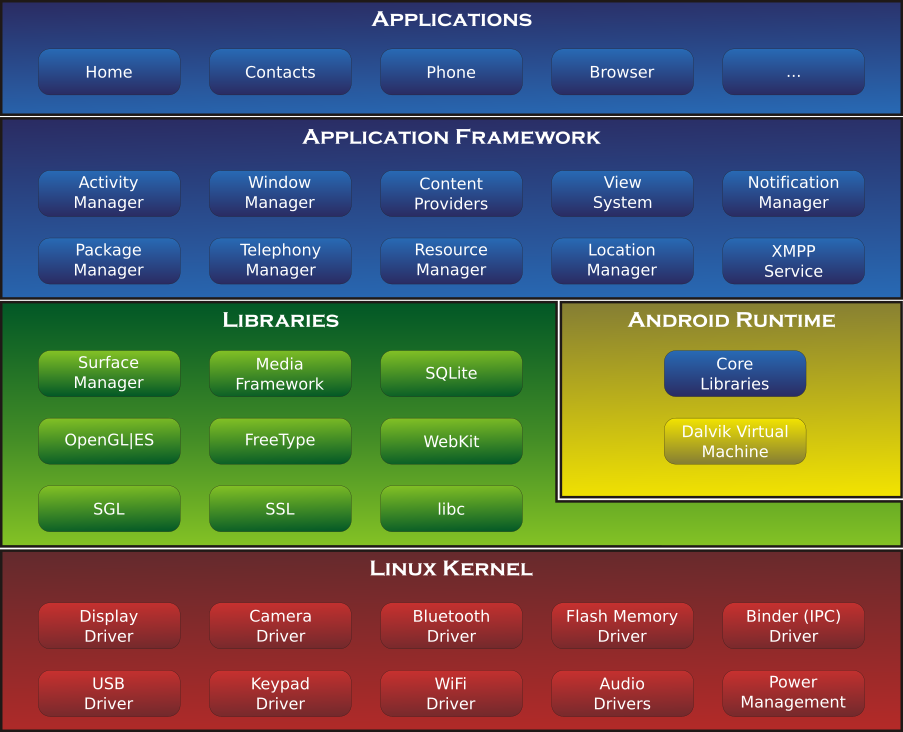
\includegraphics[scale=0.3]{android_arch.png}
    \caption{Android Software Architecture}
    \label{fig:android_arch}
\end{figure}
\end{frame}
%\begin{figure}[h!]
%  \centering
%    	\includegraphics[scale=0.5]{scada_architecture.png}
%	\caption{Architecure of a typical power SCADA system}
%	\label{scada_arch} %the label was cycle here



%\begin{figure}[h]
%  \centering
%  \begin{subfigure}[b]{1\textwidth}
%    \centering
%    \includegraphics[scale=0.4]{digraph_simple.png}
%    \caption{relation digraph of the simplified system}
%    \label{fig:digraph_simple}
%  \end{subfigure}
  
%  \begin{subfigure}[b]{1\textwidth}
%    \centering
%    \includegraphics[scale=0.4]{digraph_virtual.png}
%    \caption{Representation of the digraph with virtual nodes}
%    \label{fig:digraph_virtual}
%  \end{subfigure}
  
%\end{figure}

